\documentclass{article} % For LaTeX2e
\usepackage{nips15submit_e,times}
\usepackage{hyperref}
\usepackage{url}
\usepackage{graphicx}
\usepackage{float}
\usepackage{amsmath}
\usepackage{multirow,array}
\usepackage{listings}
\usepackage{amsfonts}
\usepackage{caption}
\usepackage{subfigure}
\usepackage{algorithm,algorithmic}

%\documentstyle[nips14submit_09,times,art10]{article} % For LaTeX 2.09
%\usepackage{fontspec}

\renewcommand{\algorithmicrequire}{ \textbf{Input:}} %Use Input in the format of Algorithm
\renewcommand{\algorithmicensure}{ \textbf{Output:}} %UseOutput in the format of Algorithm  

\definecolor{mygreen}{rgb}{0,0.6,0}
\definecolor{mygray}{rgb}{0.5,0.5,0.5}
\definecolor{mymauve}{rgb}{0.58,0,0.82}
\lstset{ %
backgroundcolor=\color{white},   % choose the background color
basicstyle=\footnotesize\ttfamily,        % size of fonts used for the code
columns=fullflexible,
breaklines=true,                 % automatic line breaking only at whitespace
captionpos=b,                    % sets the caption-position to bottom
tabsize=4,
commentstyle=\color{mygreen},    % comment style
escapeinside={\%*}{*)},          % if you want to add LaTeX within your code
keywordstyle=\color{blue},       % keyword style
stringstyle=\color{mymauve}\ttfamily,     % string literal style
frame=single,
rulesepcolor=\color{red!20!green!20!blue!20},
% identifierstyle=\color{red},
language=c++,
}

\title{Weekly Report(Apr 16,2018-Apr 22,2018)}


\author{
Liu Junnan\\
ljnsjtu@hotmail.com
}

% The \author macro works with any number of authors. There are two commands
% used to separate the names and addresses of multiple authors: \And and \AND.
%
% Using \And between authors leaves it to \LaTeX{} to determine where to break
% the lines. Using \AND forces a linebreak at that point. So, if \LaTeX{}
% puts 3 of 4 authors names on the first line, and the last on the second
% line, try using \AND instead of \And before the third author name.

\newcommand{\fix}{\marginpar{FIX}}
\newcommand{\new}{\marginpar{NEW}}

%\nipsfinalcopy % Uncomment for camera-ready version

\begin{document}


\maketitle

\begin{abstract}
This report is focused on the work I have done this week. Generally I will talk about neural network, clustering algorithms and recommender systems along with some experiments and details.
\end{abstract}

\section{Work Done}
This week I continued to learn machine learning course, including neural network, clustering algorithms and recommender systems.

\subsection{Neural Network Contd.}
A basic neural network model is shown in Fig. \ref{fig:nnmodel}. The course requires to implement neural network algorithm, including forward and back propagation processes. Although the implementation is not quite difficult given detailed instructions, a widely used trick -- vectorization is worth mentioning.

\begin{figure}[h]
%\centering
%\framebox[4.0in]{$\;$}
%\fbox{\rule[-.5cm]{0cm}{4cm} \rule[-.5cm]{4cm}{0cm}}
\begin{center}
    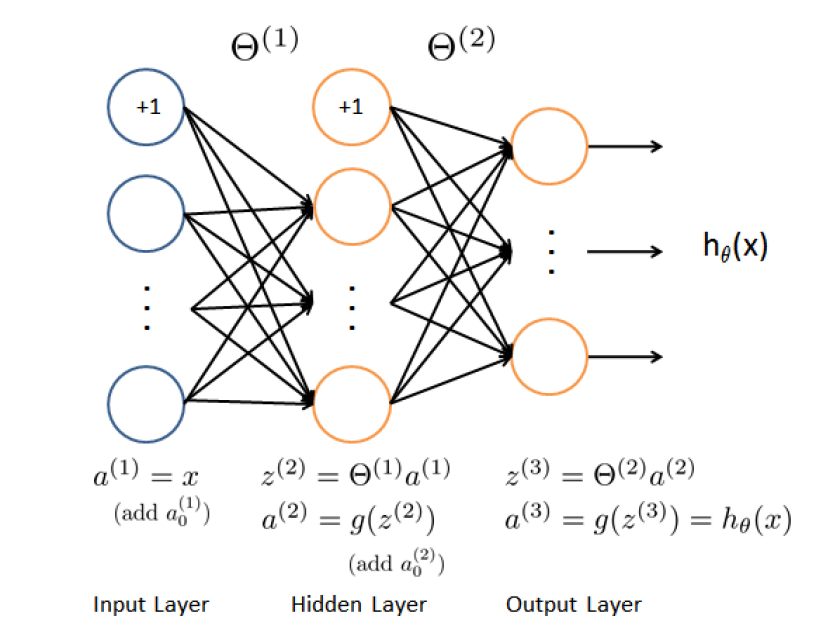
\includegraphics[width=0.6\textwidth]{nn-model.png}
\end{center}
\caption{Neural Network Model}
\label{fig:nnmodel}
$x$ denotes the input, $g(z)$ the activation function, $\Theta^{(i)}$ the weights from layer $i$ to layer $i+1$, $a^{(i)}$ the output (activation value) of neurons in layer $i$, $h_\theta(x)$ the hypothesis of input $x$, or the prediction.
\end{figure}

\subsubsection{Vectorization}
A neural network usually uses cross entropy loss function

$$J(\theta) = \frac{1}{m} \sum_{i=1}^m \sum_{k=1}^K \left[ -y_k^{(i)}\log((h_\theta(x^{(i)}))_k) + (1 - y_k^{(i)})\log(1 - h_\theta(x^{(i)})_k) \right]$$

One method is using two for-loops
\begin{lstlisting}[language=matlab]
for i=1:m
	for j=1:num_labels
		J = J + -yVec(i,j)*log(a3(i,j)) - (1-yVec(i,j)) * log(1 - a3(i,j));
	end
end
J = J / m;
\end{lstlisting}

If we use matrix computation instead of element-wise computation, the code can be shortened as one line

\begin{lstlisting}[language=matlab]
J = 1/m * sum(sum(-yVec .* log(a3) - (1 - yVec) .* log(1 - a3)));
\end{lstlisting}

Then we can use built-in timing commands tic and toc to measure the time cost. After running these part of code for 4 times, the average time interval of for-loop is $t_l = 0.004469s$, while that of vectorization is $t_v=0.002440s$, showing that $t_v/t_l=0.546$, almost half of the time saved.

Although it is just a simple experiment that compares the time cost between with or without vectorization, the result strongly suggests that we should apply vectorization wherever possible, since Matlab or any other programming languages' matrix packages highly optimize the matrix computations.

\subsection{Bias and Variance}
A machine learning algorithm sometimes suffers from over-fitting and under-fitting(shown in Fig. \ref{fig:overfit}). If the number of features are large and number of training examples small, it can overfit. A widely used method to address overfitting problem is adding a regularization term into the cost function $J$. Let's take logistic regression as an example:
$$J(\theta) = \frac{1}{m} \sum_{i=1}^m \sum_{k=1}^K \left[ -y_k^{(i)}\log((h_\theta(x^{(i)}))_k) + (1 - y_k^{(i)})\log(1 - h_\theta(x^{(i)})_k) \right] + \frac{\lambda}{2m}\sum_{j=1}^{m}\theta_j^2$$

\begin{figure}[h]
  \centering
  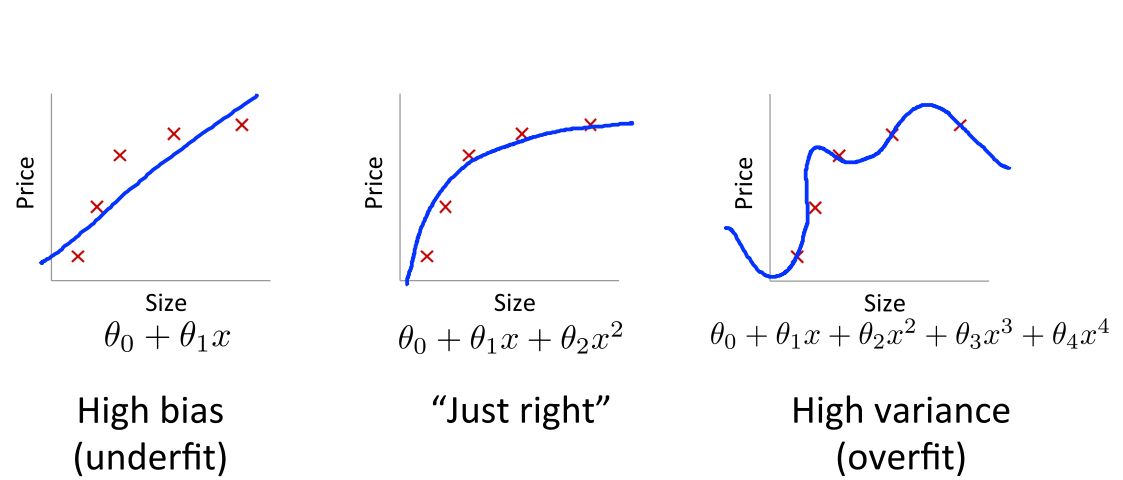
\includegraphics[width=0.9\textwidth]{under-and-over-fit.png}
  \caption{Under fitting and over fitting problem for linear regression}
  \label{fig:overfit}
\end{figure}

By changing the value of $\lambda$, the result will be different, maybe better or even worse. More concretely, given a set of examples with 2 features(shown in Fig. \ref{fig:training-data}), we want to train a logistic classifier to predict the type of a new data. After training the model, we can draw the decision boundary for visualization. If we don't use regularization technique($\lambda=0$), the decision boundary looks like Fig. \ref{fig:lambda-0}. The curve looks quite twisted but well separates positives from negatives. Apparently this model won't generalize to upcoming data. On the contrary, if we set $\lambda$ as a very huge value, it will cause underfitting(Fig. \ref{fig:lambda-100}), which can't even separate the training data. To avoid these two problems, we should try a series of different values of $\lambda$ and find the best performance. In this case, $\lambda=1$ works just fine(Fig. \ref{fig:lambda-1}).

\begin{figure}[h]
  \centering
  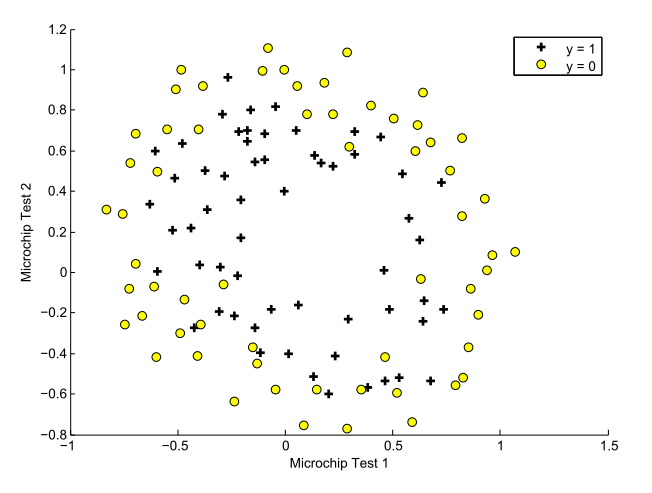
\includegraphics[width=0.6\textwidth]{training-data.png}
  \caption{Plot of training data}
  \label{fig:training-data}
\end{figure}

\begin{figure}[h]
  \centering
  % Requires \usepackage{graphicx}
  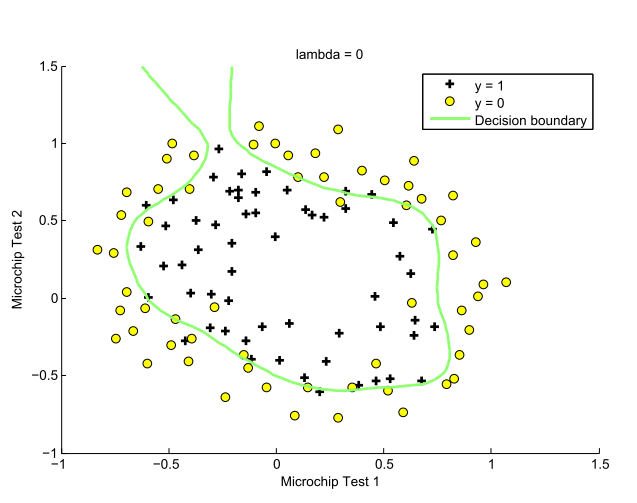
\includegraphics[width=0.6\textwidth]{lambda0}\\
  \caption{Overfitting($\lambda=0$)}\label{fig:lambda-0}
\end{figure}


\begin{figure}[h]
  \centering
  % Requires \usepackage{graphicx}
  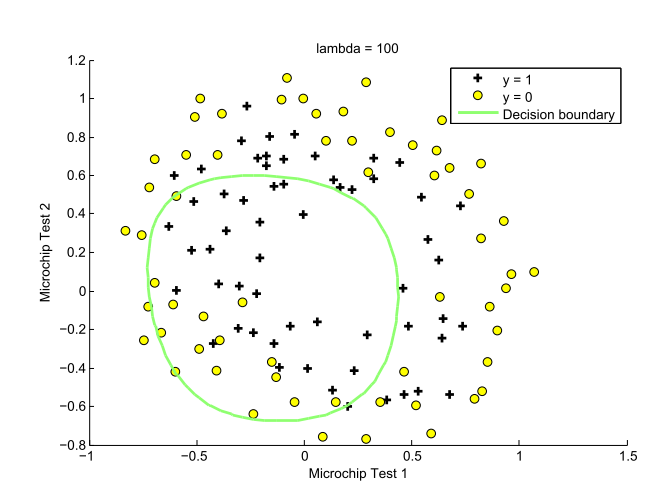
\includegraphics[width=0.6\textwidth]{lambda100}\\
  \caption{Underfitting($\lambda=100$)}\label{fig:lambda-100}
\end{figure}


\begin{figure}[h]
  \centering
  % Requires \usepackage{graphicx}
  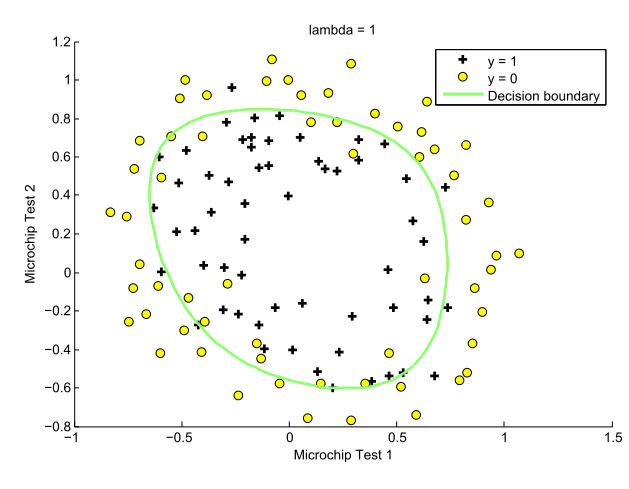
\includegraphics[width=0.6\textwidth]{lambda1}\\
  \caption{Good fitting($\lambda=1$)}\label{fig:lambda-1}
\end{figure}

\subsection{Error Metrics for Skewed Classes}
In classification tasks, we usually use accuracy as the metric of our model. But sometimes skewed classes, or unbalanced classes problems will occur, meaning that the number of negative examples overwhelms that of positive ones. In such cases, accuracy is insufficient to measure the performance of the trained models. Therefore, the confusion matrix is introduced to address this kind of problems, which is defined in Table \ref{tab:confusion-matrix}:

\begin{table}[h]
  \centering
  \begin{tabular}{|c|c|cc|}
    \hline
    \multicolumn{2}{|c|}{\multirow{2}{*}{Confusion Matrix}} & \multicolumn{2}{c|}{Predicted}\\
    \cline{3-4}
    \multicolumn{2}{|c|}{} &  0 & 1\\
    \hline
    \multicolumn{1}{|c|}{\multirow{2}{*}{Real}} & 0 & TN & FP\\
     & 1 & FN & TP\\
    \hline
  \end{tabular}
  \caption{Confusion Matrix}\label{tab:confusion-matrix}
\end{table}

Then accuracy is given as $\frac{TP+TN}{TP+TN+FP+FN}$. What's more, we define precision $p=\frac{TP}{TP+FP}$, and recall $r=\frac{TP}{TP+FN}$. By altering the value of threshold, we can get pairs of precision-recall and then draw a figure. If we want a real number to measure the performance, we have
$$F_1 \text{ score} = \frac{2*p*r}{p+r}$$
So we can compare different models with their $F_1$ scores accordingly, the more it is close to $1$, the better performance it has.

\subsection{Unsupervised Learning}
Contrary to supervised learning, the training data of unsupervised learning are not given specific labels, but we still want to partition them into several groups out of certain purpose. K-means algorithm is a typical clustering algorithm that solves the problem above, which is given in Algorithm\ref{alg:k-means},
\begin{algorithm}[H]
  \caption{K-means algorithm}
  \label{alg:k-means}
  \hspace*{0.02in} {\textbf{Input:} number of clusters $K$, $m$ training examples $\{x^{(1)}, x^{(1)}, \dots, x^{(m)}\}$} %�㷨�����룬 \hspace*{0.02in}��������λ�ã�ͬʱ���� \\ ���л���
  \begin{algorithmic}[1]
  \STATE Randomly initialize $K$ cluster centroids $\mu_1,\mu_2,\dots,\mu_K \in \mathbb{R}^n$\\
  \REPEAT 
    \FOR{$i=1$ to $m$}
        \STATE $c^{(i)}:=$ index of cluster centroid closest to $x^{(i)}$\\
    \ENDFOR
    \FOR{$k=1$ to $K$}
        \STATE $\mu_k:=$ mean of points assigned to cluster $k$
    \ENDFOR
  \UNTIL{converge}
  \end{algorithmic}
\end{algorithm}

K-means is an iterative algorithm, and the result is related to the initial values assigned to cluster centroids $\mu_1,\mu_2,\dots,\mu_K$. Sometimes different initial values will give totally different results(Shown in Fig. \ref{fig:k-means-init}). To solve this problem, we can run multiple times of K means algorithm with different initialization settings, and choose the best one.

\begin{figure}[h]
    \subfigure[good]{
        \begin{minipage}{7cm}
        \centering
        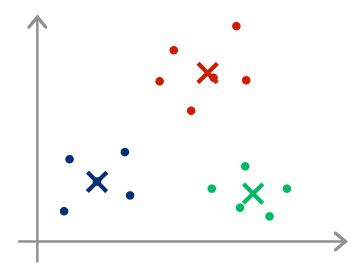
\includegraphics[width=2.2in]{good-init.png}
        \end{minipage}
    }
    \subfigure[bad]{
        \begin{minipage}{7cm}
        \centering
        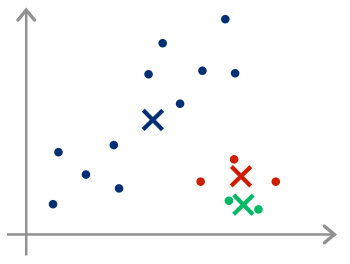
\includegraphics[width=2.2in]{bad-init.png}
        \end{minipage}
    }
  \label{fig:k-means-init}
  \caption{K-Means Initialization}
\end{figure}

\subsection{Recommender System}
Recommender systems are widely applied machine learning algorithms. For instance, a moving rating website recommends some new movies that a user has not watched yet but he will probably like them as well. The web site can apply machine learning algorithms such as content-based recommender system and collaborative filtering to achieve this job. Content-based methods are based on descriptions of the item and a profile of the user's preferences. Collaborative filtering methods are based on collecting and analyzing a large amount of information on users�� preferences and predicting what users will like based on their similarity to other users. A key advantage of the collaborative filtering approach is that it is capable of accurately recommending complex items such as movies without requiring an ``understanding'' of the item itself.

\section{Plans}
In the next week I will finish machine learning course and go on to the next step of training.

\end{document}
